\chapter{Surface Modeling and Mesh Generation}
\label{ch:surface_modeling}

%-------------------------------------------------------------
\section{B\'ezier Surfaces}
\label{sec:bezier_surface}

\subsection{Overview}
A B\'ezier surface\index{Bezier surface} is a smooth surface used in computer graphics and computer-aided design (CAD) that is controlled by a rectangular grid of points, called control points\cite{bezier1968,farin2002}. It is a 2D extension of the B\'ezier curve. The surface is defined by a pair of parameters $(u, v)$, both in the range $[0, 1]$. Evaluating a B\'ezier surface means calculating the 3D coordinates $(x, y, z)$ corresponding to a given $(u, v)$ coordinate.

\subsection{Definitions}
\begin{definition}[Control Points]\label{def:control_points}
A grid of $m+1$ by $n+1$ points $P_{ij}$ in 3D space that define the shape of the B\'ezier surface.
\end{definition}

\begin{definition}[Bernstein Polynomials]\label{def:bernstein_polynomials}
The basis functions $B_{i,n}(t) = \binom{n}{i} t^i (1-t)^{n-i}$ used to weight the control points in B\'ezier surface evaluation.
\end{definition}

\begin{definition}[Tensor Product]\label{def:tensor_product}
The method of forming a surface by multiplying two orthogonal B\'ezier curves, i.e., $Q(u,v) = \sum_{i,j} B_{i,m}(u) B_{j,n}(v) P_{ij}$.
\end{definition}

\begin{definition}[de Casteljau's Algorithm]\label{def:de_casteljau}
A recursive algorithm for evaluating B\'ezier curves and surfaces that is numerically stable and geometrically intuitive.
\end{definition}

\subsection{Theory}
A B\'ezier surface point $Q(u, v)$ is calculated using the formula:
$$Q(u, v) = \sum_{i=0}^m \sum_{j=0}^n B_{i,m}(u) B_{j,n}(v) P_{i,j}$$
The most efficient way to evaluate this is by using \textbf{de Casteljau's algorithm}\cite{farin2002} in two steps:
\begin{enumerate}
\item Evaluate $m+1$ separate B\'ezier curves in the $v$-direction using parameter $v$. This produces a temporary set of control points $P'_0, \dots, P'_m$ that depend only on $v$.
\item Evaluate the single B\'ezier curve defined by $P'_i$ using parameter $u$.
\end{enumerate}

This ``tensor product'' approach effectively reduces the surface evaluation to several simpler curve evaluations.

\begin{example}[Bicubic B\'ezier Surface Evaluation]\label{ex:bezier_surface}
Consider a $4 \times 4$ bicubic B\'ezier surface (degree $m = n = 3$) with 16 control points forming a $4 \times 4$ grid. To evaluate at $(u, v) = (0.25, 0.75)$:
\begin{enumerate}
    \item For each of the 4 rows, apply de Casteljau's algorithm in the $v$-direction with $v = 0.75$, producing 4 intermediate points $P'_0, P'_1, P'_2, P'_3$.
    \item Apply de Casteljau's algorithm to $P'_0, \ldots, P'_3$ in the $u$-direction with $u = 0.25$, yielding the final 3D point $Q(0.25, 0.75)$.
\end{enumerate}
Each de Casteljau step requires $O(m)$ linear interpolations, so the total cost is $O(m \cdot n)$ per evaluation.
\end{example}

\begin{figure}[htbp]
\centering
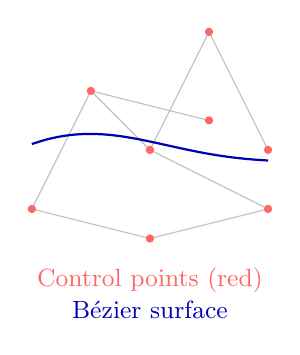
\begin{tikzpicture}[scale=0.75]
  \draw[gray!50,thin] (0,0)--(1,2)--(2,1)--(3,3)--(4,1);
  \draw[gray!50,thin] (0,0)--(2,-0.5)--(4,0);
  \draw[gray!50,thin] (1,2)--(3,1.5);
  \draw[gray!50,thin] (2,1)--(4,0);
  \foreach \x/\y in {0/0, 1/2, 2/1, 3/3, 4/1, 2/-0.5, 4/0, 3/1.5} {
    \fill[red!60] (\x,\y) circle (2pt);
  }
  \draw[blue!70!black,thick] plot[smooth,domain=0:4,samples=20] (\x,{0.8+0.5*sin(\x*40)+0.3*cos(\x*60)});
  \node[font=\small,red!60] at (2,-1.2) {Control points (red)};
  \node[font=\small,blue!70!black] at (2,-1.7) {B\'ezier surface};
\end{tikzpicture}
\caption{B\'ezier surface: a tensor-product surface defined by a control net of points.}
\label{fig:bezier_surface}
\end{figure}


\subsection{Pseudocode}
\begin{algorithm}
\caption{Evaluate B\'ezier Surface}
\label{alg:evaluate_bezier_surface}
\begin{algorithmic}[1]
\Function{EvaluateBezierSurface}{control\_points, u, v}
    \State $m \gets \text{num\_rows} - 1$
    \State $n \gets \text{num\_cols} - 1$
    \Comment{Reduce in the $v$ direction}
    \State $\text{temp\_points} \gets \emptyset$
    \For{$i \gets 0$ \textbf{to} $m$}
        \State $\text{row} \gets \text{control\_points}[i]$
        \State \Call{EvaluateBezierCurve}{\text{row}, v}
        \State $\text{temp\_points}.append(p')$
    \EndFor
    \Comment{Reduce in the $u$ direction}
    \State \Return \textbf{EvaluateBezierCurve}(temp\_points, $u$)
\EndFunction

\Function{EvaluateBezierCurve}{points, $t$}
    \State $\text{current} \gets \text{points}[:]$
    \While{$|\text{current}| > 1$}
        \State $\text{next\_level} \gets \emptyset$
        \For{$i \gets 0$ \textbf{to} $|\text{current}| - 2$}
            \State $p \gets (1 - t) \cdot \text{current}[i] + t \cdot \text{current}[i+1]$
            \State $\text{next\_level}.append(p)$
        \EndFor
        \State $\text{current} \gets \text{next\_level}$
    \EndWhile
    \State \Return $\text{current}[0]$
\EndFunction
\end{algorithmic}
\end{algorithm}

\subsection{Parameter Selection}
\begin{itemize}
\item \textbf{Parameter Range}: Parameters $u, v$ must be strictly within $[0, 1]$.
\item \textbf{Order}: The number of control points is $(m+1) \times (n+1)$. Typically $m=3, n=3$ for bicubic surfaces.
\end{itemize}

\subsection{Complexity}
\begin{itemize}
\item \textbf{Time Complexity}: $O(m \cdot n^2 + m^2)$ using the two-step de Casteljau approach. For bicubic surfaces ($m=3, n=3$), this is a small constant.
\item \textbf{Space Complexity}: $O(m \cdot n)$ to store the control point grid.
\end{itemize}

\subsection{Usages}
\begin{itemize}
\item \textbf{CAD (Computer Aided Design)}: Modeling car bodies, aircraft wings, and consumer products.
\item \textbf{Animation}: Smooth character skinning and facial deformations.
\item \textbf{TrueType/PostScript Fonts}: While fonts are 2D curves, they can be interpreted as 1D surfaces.
\item \textbf{Geometric Design}: Creating smooth transitions (blends) between different parts of a model.
\item \textbf{Fluid Simulation}: Representing the surface of a liquid with a set of smooth patches.
\end{itemize}

\subsection{Testing Methods and Edge Cases}
\begin{itemize}
\item \textbf{Corners}: Verify that $Q(0,0), Q(0,1), Q(1,0), Q(1,1)$ exactly match the four corner control points.
\item \textbf{Flat Surface}: If all control points lie on a plane, the entire evaluated surface must lie on that plane.
\item \textbf{Degree Elevation}: Increasing the number of control points without changing the surface shape.
\item \textbf{Precision}: Ensure the surface remains smooth and doesn't ``break'' at $u, v \approx 0.5$.
\item \textbf{Continuity}: Checking that adjacent B\'ezier patches meet smoothly (G1 or C1 continuity).
\end{itemize}

\subsection{References}
\begin{itemize}
\item B\'ezier, P. \cite{bezier1968} ``How Renault Uses Numerical Control for Car Body Design and Tooling''. SAE paper.
\item Farin, G. \cite{farin2002} ``Curves and Surfaces for CAGD: A Practical Guide''. Morgan Kaufmann.
\item Piegl, L., \& Tiller, W. \cite{piegl1997} ``The NURBS Book''. Springer.
\item Wikipedia: \href{https://en.wikipedia.org/wiki/B\%C3\%A9zier_surface}{B\'ezier surface}
\end{itemize}

%-------------------------------------------------------------
\section{NURBS Surfaces}
\label{sec:nurbs_surface}

\subsection{Overview}
\index{NURBS}NURBS (Non-Uniform Rational B-Splines) are a mathematical model commonly used in computer graphics and computer-aided design (CAD) for generating and representing curves and surfaces\cite{piegl1997}. NURBS surfaces provide a highly flexible and unified way to represent both analytic shapes (like spheres, cones, and cylinders) and complex, free-form organic shapes. Evaluating a NURBS surface involves calculating the 3D coordinates $(x, y, z)$ at a given parameter pair $(u, v)$ within the surface's domain.

\subsection{Definitions}
\begin{definition}[Knot Vector]\label{def:knot_vector}
A non-decreasing sequence of real numbers $t_0 \leq t_1 \leq \cdots \leq t_{n+p+1}$ that determines how the control points affect the NURBS surface.
\end{definition}

\begin{definition}[NURBS Weights]\label{def:nurbs_weights}
A scalar $w_{ij} > 0$ associated with each control point $P_{ij}$. A higher weight ``pulls'' the surface closer to that control point.
\end{definition}

\begin{definition}[B-Spline Basis Functions]\label{def:bspline_basis}
Piecewise polynomial functions $N_{i,p}$ of degree $p$ defined over a knot vector via the Cox-de Boor recursion formula.
\end{definition}

\begin{definition}[Rational Surface]\label{def:rational_surface}
The term ``rational'' refers to the use of weights and a division step, allowing for the exact representation of conic sections (circles, ellipses).
\end{definition}

\subsection{Theory}
A point on a NURBS surface $S(u, v)$ is defined as:
$$S(u, v) = \frac{\sum_{i=0}^n \sum_{j=0}^m N_{i,p}(u) N_{j,q}(v) w_{i,j} P_{i,j}}{\sum_{i=0}^n \sum_{j=0}^m N_{i,p}(u) N_{j,q}(v) w_{i,j}}$$
where $P_{i,j}$ are the control points, $w_{i,j}$ are weights, and $N_{i,p}, N_{j,q}$ are the B-spline basis functions of degrees $p$ and $q$.

The calculation typically follows these steps:
\begin{enumerate}
\item \textbf{Locate Knots}: Find the indices of the knots $u$ and $v$ in their respective knot vectors.
\item \textbf{Evaluate Basis Functions}: Compute the values of all non-zero basis functions at $u$ and $v$ using the \index{Cox-de Boor recursion}Cox-de Boor recursion formula.
\item \textbf{Summation}: Compute the weighted sum of the control points and the sum of the weights.
\item \textbf{Division}: Divide the weighted point sum by the total weight to find the final 3D point.
\end{enumerate}

\begin{example}[NURBS Circle Representation]\label{ex:nurbs_circle}
A circle of radius $r$ can be exactly represented by a single quadratic NURBS curve ($p = 2$) with 9 control points and a specific knot vector. The key insight is that the weights $w_i$ for the control points at the cardinal directions are $\cos(\pi/4) = \sqrt{2}/2$, while the weights for the diagonal control points are 1. This rational weighting is what allows NURBS to represent conic sections exactly, which polynomial B\'ezier curves cannot do.
\end{example}

\subsection{Pseudocode}
\begin{algorithm}
\caption{Evaluate NURBS Surface}
\label{alg:evaluate_nurbs_surface}
\begin{algorithmic}[1]
\Function{EvaluateNURBSSurface}{control\_points, weights, knots\_u, knots\_v, $p$, $q$, $u$, $v$}
    \State \Call{FindKnotSpan}{$n$, $p$, $u$, $\text{knots\_u}$}
    \State \Call{FindKnotSpan}{$m$, $q$, $v$, $\text{knots\_v}$}
    \State \Call{BasisFunctions}{$\text{span\_u}$, $u$, $p$, $\text{knots\_u}$}
    \State \Call{BasisFunctions}{$\text{span\_v}$, $v$, $q$, $\text{knots\_v}$}
    \State $\text{sum\_wp} \gets \mathbf{0}$
    \State $\text{sum\_w} \gets 0$
    \For{$l \gets 0$ \textbf{to} $q$}
        \State $\text{temp} \gets \mathbf{0}$
        \State $\text{temp\_w} \gets 0$
        \For{$k \gets 0$ \textbf{to} $p$}
            \State $\text{idx\_u} \gets \text{span\_u} - p + k$
            \State $\text{idx\_v} \gets \text{span\_v} - q + l$
            \State $w \gets \text{weights}[\text{idx\_u}][\text{idx\_v}]$
            \State $p_\text{val} \gets \text{control\_points}[\text{idx\_u}][\text{idx\_v}]$
            \State $\text{sum\_wp} \gets \text{sum\_wp} + N_u[k] \cdot N_v[l] \cdot w \cdot p_\text{val}$
            \State $\text{sum\_w} \gets \text{sum\_w} + N_u[k] \cdot N_v[l] \cdot w$
        \EndFor
    \EndFor
    \State \Return $\text{sum\_wp} \,/\, \text{sum\_w}$
\EndFunction
\end{algorithmic}
\end{algorithm}

\subsection{Parameter Selection}
\begin{itemize}
\item \textbf{Degree ($p, q$)}: Usually $p=3, q=3$ (bicubic) for smooth modeling.
\item \textbf{Knot Vector Type}: \textbf{Clamped} knot vectors (where the first and last $p+1$ knots are identical) ensure the surface passes exactly through its corner control points.
\end{itemize}

\subsection{Complexity}
\begin{itemize}
\item \textbf{Time Complexity}: $O(p^2 + q^2)$ to evaluate the basis functions, plus $O(p \cdot q)$ for the final summation. This is extremely efficient for low degrees.
\item \textbf{Space Complexity}: $O(n \cdot m)$ to store the control point and weight grids.
\end{itemize}

\subsection{Usages}
\begin{itemize}
\item \textbf{Industrial CAD}: Standard data format (IGES, STEP) for exchanging 3D models between different engineering software (SolidWorks, Rhino, CATIA).
\item \textbf{Reverse Engineering}: Fitting smooth surfaces to scanned point cloud data.
\item \textbf{Scientific Visualization}: Smoothly interpolating scattered spatial data (e.g., bathymetry or atmospheric pressure).
\item \textbf{High-End Animation}: Rendering complex character models (Pixar's RenderMan uses NURBS extensively).
\item \textbf{Naval Architecture}: Designing boat hulls for optimal fluid flow.
\end{itemize}

\subsection{Testing Methods and Edge Cases}
\begin{itemize}
\item \textbf{Analytic Shapes}: Verify that a NURBS surface with appropriate weights can exactly represent a sphere or a cylinder.
\item \textbf{Weights of 1}: If all weights are 1.0, the surface must behave identically to a non-rational B-spline surface.
\item \textbf{Boundary Conditions}: Verify that the surface interpolates its corner control points (for clamped knots).
\item \textbf{Numerical Stability}: Ensure the denominator (total weight) does not approach zero.
\item \textbf{Derivative Calculation}: Verify that the surface normals (calculated from $u$ and $v$ derivatives) are smooth and consistent.
\end{itemize}

\subsection{References}
\begin{itemize}
\item Piegl, L., \& Tiller, W. \cite{piegl1997} ``The NURBS Book''. Springer.
\item Rogers, D. F. (2001). ``An Introduction to NURBS: With Historical Perspective''. Morgan Kaufmann.
\item Farin, G. \cite{farin2002} ``Curves and Surfaces for CAGD: A Practical Guide''. Morgan Kaufmann.
\item Wikipedia: \href{https://en.wikipedia.org/wiki/Non-uniform_rational_B-spline}{Non-uniform rational B-spline}
\end{itemize}

%-------------------------------------------------------------
\section{Mesh Voxelization}
\label{sec:mesh_voxelization}

\subsection{Overview}
\index{voxelization}Mesh voxelization is the process of converting a 3D surface mesh (typically composed of triangles) into a volumetric representation called a \textbf{voxel grid}\cite{akeninemoller2001,nooruddin2003}. A voxel (volume element) is the 3D equivalent of a pixel. Voxelization is used to simplify complex geometry, perform volumetric analysis, and prepare models for physics simulations or 3D printing. The process can result in a ``binary'' voxel grid (occupied vs.\ empty) or a ``solid'' voxelization (distinguishing interior from exterior).

\subsection{Definitions}
\begin{definition}[Voxel]\label{def:voxel}
A unit of volume on a regular 3D grid.
\end{definition}

\begin{definition}[Conservative Voxelization]\label{def:conservative_voxelization}
A method that ensures a voxel is marked as occupied if any part of the triangle passes through it.
\end{definition}

\begin{definition}[Parity Rule]\label{def:parity_rule}
A technique for solid voxelization where a voxel's ``insideness'' is determined by counting intersections of a ray with the mesh boundary using the even-odd rule.
\end{definition}

\subsection{Theory}
The most common approach to surface voxelization is based on \index{triangle-box intersection}\textbf{triangle-box intersection} tests\cite{akeninemoller2001}.
\begin{enumerate}
\item Define a 3D grid that encloses the mesh's bounding box.
\item For each triangle in the mesh:
  \begin{itemize}
  \item Determine the range of voxels it might intersect (its AABB in grid coordinates).
  \item For every voxel in that range, perform a rigorous triangle-box intersection test (e.g., using the Akenine-M\"oller algorithm based on the Separating Axis Theorem).
  \end{itemize}
\item To perform \textbf{solid voxelization} (filling the interior):
  \begin{itemize}
  \item After surface voxelization, use a flood-fill algorithm starting from the grid boundaries to identify ``outside'' voxels\cite{nooruddin2003}.
  \item Everything not reachable from the outside is ``inside.''
  \item Alternatively, use ray-casting along each grid line and apply the even-odd rule.
  \end{itemize}
\end{enumerate}

\begin{example}[Voxelizing a Cube]\label{ex:voxelize_cube}
Consider a unit cube (8 vertices, 12 triangular faces) voxelized at resolution $8 \times 8 \times 8$. The bounding box is $[0,1]^3$ with voxel size $1/8$. Each of the 12 triangles is tested against its AABB in grid coordinates. Surface voxels on each face are marked. Then flood-fill from a corner voxel identifies all voxels on the exterior. The remaining interior voxels form a $6 \times 6 \times 6$ solid block of 216 inside voxels (the boundary voxels separate inside from outside).
\end{example}

\subsection{Pseudocode}
\begin{algorithm}
\caption{Voxelize Mesh}
\label{alg:voxelize_mesh}
\begin{algorithmic}[1]
\Function{VoxelizeMesh}{mesh, resolution}
    \State $\text{bbox} \gets \text{mesh.GetBoundingBox()}$
    \State $\text{voxel\_size} \gets \text{bbox.size}.\max() \,/\, \text{resolution}$
    \State $\text{grid} \gets \text{array}[\text{resolution}]^3$ initialized to \textsc{Empty}
    \Comment{Surface Voxelization}
    \For{\textbf{each} $\text{triangle}$ \textbf{in} mesh.faces}
        \State \Call{WorldToGrid}{\text{triangle.min}, \text{bbox}, \text{voxel\_size}}
        \State \Call{WorldToGrid}{\text{triangle.max}, \text{bbox}, \text{voxel\_size}}
        \For{$x \gets \text{min\_v}.x$ \textbf{to} $\text{max\_v}.x$}
            \For{$y \gets \text{min\_v}.y$ \textbf{to} $\text{max\_v}.y$}
                \For{$z \gets \text{min\_v}.z$ \textbf{to} $\text{max\_v}.z$}
                    \State \Call{GetVoxelBox}{x, y, z, \text{bbox}, \text{voxel\_size}}
                    \If{\Call{TriangleBoxIntersect}{triangle, voxel\_box}}
                        \State $\text{grid}[x][y][z] \gets \textsc{Surface}$
                    \EndIf
                \EndFor
            \EndFor
        \EndFor
    \EndFor
    \Comment{Solid Voxelization (Optional)}
    \State \Call{FloodFill}{grid, start\_pos$=(0,0,0)$, target=\textsc{Empty}, replacement=\textsc{Outside}}
    \For{$(x, y, z)$ \textbf{in} grid}
        \If{$\text{grid}[x][y][z] = \textsc{Empty}$}
            \State $\text{grid}[x][y][z] \gets \textsc{Inside}$
        \EndIf
    \EndFor
    \State \Return grid
\EndFunction
\end{algorithmic}
\end{algorithm}

\subsection{Parameter Selection}
\begin{itemize}
\item \textbf{Resolution}: Higher resolution captures more detail but increases memory consumption cubically ($O(N^3)$).
\item \textbf{Intersection Strategy}: Conservative voxelization is preferred for tasks like collision detection to avoid ``gaps'' in the surface.
\end{itemize}

\subsection{Complexity}
\begin{itemize}
\item \textbf{Time Complexity}: $O(F \cdot K^3)$ where $F$ is the face count and $K$ is the local grid size per triangle. For solid filling, $O(N^3)$ where $N$ is the resolution.
\item \textbf{Space Complexity}: $O(N^3)$ to store the 3D grid. Sparse representations like \textbf{OpenVDB} or \textbf{Octrees} can reduce this significantly.
\end{itemize}

\subsection{Usages}
\begin{itemize}
\item \textbf{3D Printing}: Slicing software voxelizes models to generate toolpaths and infill patterns.
\item \textbf{Physics Simulation}: Converting complex meshes into voxels for fluid dynamics (Lattice Boltzmann Method) or smoke simulation.
\item \textbf{Collision Detection}: Using a voxel grid as a spatial index for fast intersection queries.
\item \textbf{Medical Imaging}: Modeling organs or bones from surface scans for surgical planning.
\item \textbf{Game Development}: Destructible environments (e.g., Minecraft or Teardown) and GPU-based global illumination.
\end{itemize}

\subsection{Testing Methods and Edge Cases}
\begin{itemize}
\item \textbf{Watertightness}: Verify that solid voxelization produces no ``leaks'' for a closed mesh.
\item \textbf{Thin Features}: Ensure triangles thinner than a voxel are still captured (conservative test).
\item \textbf{Non-Manifold Mesh}: Test how the solid filler handles meshes with holes (usually results in the entire model being marked as outside).
\item \textbf{Numerical Precision}: Triangle-box tests are sensitive to floating-point errors; use robust epsilon values.
\item \textbf{Memory Limit}: Check performance and stability at high resolutions (e.g., $1024^3$).
\end{itemize}

\subsection{References}
\begin{itemize}
\item Akenine-M\"oller, T. \cite{akeninemoller2001} ``Fast 3D Triangle-Box Overlap Testing''. Journal of Graphics Tools.
\item Nooruddin, F. S., \& Turk, G. \cite{nooruddin2003} ``Simplification and Repair of Polygonal Models Using Volumetric Techniques''. IEEE TVCG.
\item Schwarz, M., \& Seidel, H. P. (2010). ``Fast Parallel Surface and Solid Voxelization on GPUs''. ACM TOG.
\item Wikipedia: \href{https://en.wikipedia.org/wiki/Voxel}{Voxel}
\end{itemize}

%-------------------------------------------------------------
\section{Winding-Filtered Tetrahedral Meshing}
\label{sec:winding_filtered_tet_meshing}

\subsection{Overview}
Winding-Filtered Tetrahedral Meshing is a robust technique for generating a volumetric tetrahedral mesh from a surface mesh, even if the surface mesh is ``dirty'' (i.e., contains self-intersections or holes)\cite{hu2018}.

Traditional tetrahedralization algorithms (like constrained Delaunay) often require a clean, manifold surface. In contrast, winding-filtered meshing uses the \index{generalized winding number}Generalized Winding Number (GWN) to classify tetrahedra as interior or exterior, which is robust even for non-manifold inputs.

\subsection{Implementation Details}
In \texttt{CompGeom}, the \texttt{WindingFilteredTetMesher} uses the following process (inspired by fTetWild\cite{hu2018}):
\begin{enumerate}
\item \textbf{Bounding Box Expansion}: Create a large super-tetrahedron containing the entire surface mesh.
\item \textbf{Point Insertion}: Add surface vertices and a dense grid of internal Steiner points to the tetrahedralization.
\item \textbf{Delaunay Tetrahedralization}: Construct a global Delaunay tetrahedralization of the point set.
\item \textbf{Winding-Based Filtering}: For each tetrahedron, compute the Generalized Winding Number of its centroid with respect to the original surface mesh.
\item \textbf{Output}: Retain only tetrahedra where the GWN $> 0.5$ (indicating the interior of the domain).
\end{enumerate}

\begin{example}[Winding Number Classification]\label{ex:winding_number}
Consider a closed tetrahedron surface mesh. For a point inside the tetrahedron, the generalized winding number is 1.0 (the surface wraps around it exactly once). For a point outside, the winding number is 0.0. The threshold of 0.5 cleanly separates interior from exterior. Even if the surface has a small gap (non-watertight), the winding number degrades gracefully, correctly classifying most interior tetrahedra.
\end{example}

\subsection{Usage}
\begin{algorithm}
\caption{Winding-Filtered Tet Meshing}
\label{alg:winding_filtered_tet}
\begin{algorithmic}[1]
\State \texttt{from compgeom.mesh.volume.tetmesh.winding\_filtered\_mesher import WindingFilteredTetMesher}
\State \texttt{import numpy as np}
\State
\Comment{surface vertices and faces as numpy arrays}
\State $\text{vertices} \gets \texttt{np.array}([[0,0,0], [1,0,0], [0,1,0], [0,0,1]])$
\State $\text{faces} \gets \texttt{np.array}([[0,1,2], [0,2,3], [0,3,1], [1,2,3]])$
\State
\State \Call{WindingFilteredTetMesher}{\text{vertices}, \text{faces}}
\State $\text{tet\_mesh} \gets \text{mesher.mesh(refinement\_factor=1.0)}$
\end{algorithmic}
\end{algorithm}

\subsection{References}
\begin{itemize}
\item Hu, Y., et al. ``fTetWild: Robust Tetrahedral Meshing in the Wild.'' ACM Transactions on Graphics (SIGGRAPH), 2018.
\item Jacobson, A., et al. ``Robust Inside-Outside Segmentation using Generalized Winding Numbers.'' ACM Transactions on Graphics (SIGGRAPH), 2013.
\end{itemize}

%-------------------------------------------------------------
\section{Mesh Refinement}
\label{sec:mesh_refinement}

\subsection{Overview}
\index{mesh refinement}Mesh refinement is the process of increasing the resolution of a mesh by subdividing its elements (faces and edges) into smaller ones. The goal is to improve the mesh's quality, accuracy for numerical simulations, or visual smoothness\cite{loop1987,catmull1978}. Refinement can be \textbf{global} (applied to the entire mesh) or \textbf{local} (applied only to specific regions of interest). Common algorithms include Loop subdivision (for triangles) and Catmull-Clark subdivision (for quads).

\subsection{Definitions}
\begin{definition}[Subdivision]\label{def:subdivision}
Splitting an existing face into multiple smaller faces.
\end{definition}

\begin{definition}[Edge Split]\label{def:edge_split}
Inserting a new vertex at the midpoint of an edge and splitting the edge into two.
\end{definition}

\begin{definition}[Face Split]\label{def:face_split}
Connecting a new vertex at the centroid of a face to its original vertices.
\end{definition}

\begin{definition}[Adaptive Refinement]\label{def:adaptive_refinement}
Refinement that occurs only where a specific error metric exceeds a threshold.
\end{definition}

\begin{definition}[Stencil]\label{def:stencil}
A weighted average formula used to determine the position of new and original vertices after subdivision.
\end{definition}

\subsection{Theory}
Most refinement schemes follow a two-step process:
\begin{enumerate}
\item \textbf{Topological Split}: The mesh connectivity is modified to create more faces (e.g., 1-to-4 triangle split).
\item \textbf{Smoothing (Geometric Update)}: The positions of the new and existing vertices are adjusted based on their neighbors to achieve a specific level of smoothness (e.g., $C^1$ or $C^2$ continuity).
\end{enumerate}

For example, in \textbf{Loop Subdivision}\cite{loop1987}:
\begin{itemize}
\item Each triangle is split into four smaller triangles.
\item New ``edge vertices'' are positioned using a weighted average of the endpoints and the opposite vertices of the two incident faces.
\item Original ``even vertices'' are repositioned based on their neighbors to maintain surface smoothness.
\end{itemize}

For \textbf{Catmull-Clark Subdivision}\cite{catmull1978}:
\begin{itemize}
\item Each quad is split into four smaller quads by inserting vertices at face centers and edge midpoints.
\item The limiting surface is $C^2$ everywhere except at extraordinary vertices (where $C^1$ continuity holds).
\end{itemize}

\begin{example}[1-to-4 Triangle Refinement]\label{ex:triangle_refinement}
Start with a single equilateral triangle with vertices $A$, $B$, $C$. After one level of 1-to-4 refinement:
\begin{itemize}
    \item Three new edge midpoints are created: $M_{AB}$, $M_{BC}$, $M_{CA}$.
    \item Four new triangles are formed: $(A, M_{AB}, M_{CA})$, $(B, M_{BC}, M_{AB})$, $(C, M_{CA}, M_{BC})$, $(M_{AB}, M_{BC}, M_{CA})$.
    \item The number of faces goes from 1 to 4, edges from 3 to 9, and vertices from 3 to 6.
    \item The Euler characteristic is preserved: $\chi = 6 - 9 + 4 = 1$ (disk), same as the original $\chi = 3 - 3 + 1 = 1$.
\end{itemize}
\end{example}

\begin{figure}[htbp]
\centering
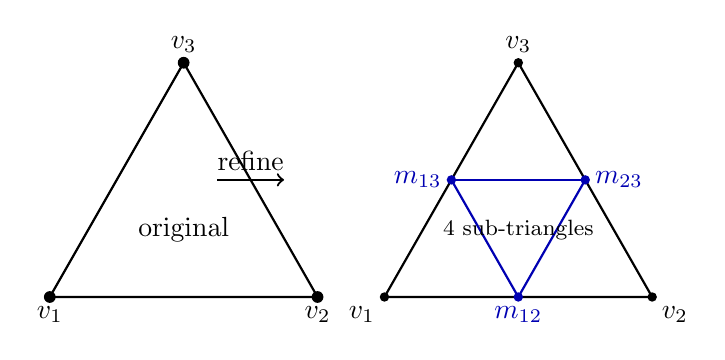
\begin{tikzpicture}[scale=0.85]
  \begin{scope}[xshift=-3cm]
    \draw[thick] (0,0)--(4,0)--(2,3.5)--cycle;
    \fill (0,0) circle (2.5pt) node[below] {$v_1$};
    \fill (4,0) circle (2.5pt) node[below] {$v_2$};
    \fill (2,3.5) circle (2.5pt) node[above] {$v_3$};
    \node at (2,1) {original};
  \end{scope}
  \draw[->,thick] (-0.5,1.75)--(0.5,1.75);
  \node[above] at (0,1.75) {refine};
  \begin{scope}[xshift=2cm]
    \draw[thick] (0,0)--(4,0)--(2,3.5)--cycle;
    \draw[blue!70!black,thick] (2,0)--(3,1.75);
    \draw[blue!70!black,thick] (1,1.75)--(3,1.75);
    \draw[blue!70!black,thick] (1,1.75)--(2,0);
    \fill (0,0) circle (2pt) node[below left] {$v_1$};
    \fill (4,0) circle (2pt) node[below right] {$v_2$};
    \fill (2,3.5) circle (2pt) node[above] {$v_3$};
    \fill[blue!70!black] (2,0) circle (2pt) node[below] {$m_{12}$};
    \fill[blue!70!black] (3,1.75) circle (2pt) node[right] {$m_{23}$};
    \fill[blue!70!black] (1,1.75) circle (2pt) node[left] {$m_{13}$};
    \node at (2,1) {\footnotesize 4 sub-triangles};
  \end{scope}
\end{tikzpicture}
\caption{1-to-4 triangle refinement: each edge is split at its midpoint, producing four congruent sub-triangles.}
\label{fig:mesh_refinement}
\end{figure}


\subsection{Pseudocode: Simple 1-to-4 Triangle Refinement}
\begin{algorithm}
\caption{Refine Mesh}
\label{alg:refine_mesh}
\begin{algorithmic}[1]
\Function{RefineMesh}{mesh}
    \State $\text{new\_vertices} \gets \text{mesh.vertices}[:]$
    \State $\text{new\_faces} \gets \emptyset$
    \State $\text{edge\_midpoints} \gets \{\}$
    \Comment{Create new vertices at every edge midpoint}
    \For{\textbf{each} $\text{edge}$ \textbf{in} mesh.edges}
        \State $(v_1, v_2) \gets \text{edge}$
        \State $\text{mid\_p} \gets (\text{mesh.vertices}[v_1] + \text{mesh.vertices}[v_2]) \,/\, 2.0$
        \State $\text{edge\_midpoints}[\text{sorted}(\text{edge})] \gets |\text{new\_vertices}|$
        \State $\text{new\_vertices}.append(\text{mid\_p})$
    \EndFor
    \Comment{Create four new triangles for every original face}
    \For{\textbf{each} $\text{face}$ \textbf{in} mesh.faces}
        \State $(v_1, v_2, v_3) \gets \text{face}$
        \State $m_1 \gets \text{edge\_midpoints}[\text{sorted}(v_1, v_2)]$
        \State $m_2 \gets \text{edge\_midpoints}[\text{sorted}(v_2, v_3)]$
        \State $m_3 \gets \text{edge\_midpoints}[\text{sorted}(v_3, v_1)]$
        \State $\text{new\_faces}.append((v_1, m_1, m_3))$
        \State $\text{new\_faces}.append((v_2, m_2, m_1))$
        \State $\text{new\_faces}.append((v_3, m_3, m_2))$
        \State $\text{new\_faces}.append((m_1, m_2, m_3))$
    \EndFor
    \State \Return \Call{Mesh}{new\_vertices, new\_faces}
\EndFunction
\end{algorithmic}
\end{algorithm}

\subsection{Parameter Selection}
\begin{itemize}
\item \textbf{Refinement Level}: The number of iterations. Each iteration of 1-to-4 split quadruples the number of faces.
\item \textbf{Metric}: For adaptive refinement, common metrics include curvature, gradient of a simulated field (e.g., stress or temperature), or edge length.
\end{itemize}

\subsection{Complexity}
\begin{itemize}
\item \textbf{Time Complexity}: $O(F \cdot 4^k)$ where $F$ is the original face count and $k$ is the refinement level.
\item \textbf{Space Complexity}: $O(F \cdot 4^k)$ to store the refined mesh.
\end{itemize}

\subsection{Usages}
\begin{itemize}
\item \textbf{Computer Graphics}: Generating high-fidelity models from low-poly base meshes (e.g., characters in movies or games).
\item \textbf{Finite Element Method (FEM)}: Improving solution accuracy in regions with high stress or fluid turbulence.
\item \textbf{3D Printing}: Increasing the resolution of a mesh to ensure smooth curved surfaces after slicing.
\item \textbf{Terrain Modeling}: Adding detail to a coarse elevation grid where the landscape is complex.
\item \textbf{Surface Reconstruction}: Improving the density of a mesh fitted to a sparse point cloud.
\end{itemize}

\subsection{Testing Methods and Edge Cases}
\begin{itemize}
\item \textbf{Consistency}: Verify that the refined mesh occupies the exact same volume as the original (for linear refinement).
\item \textbf{Manifold Property}: Ensure refinement doesn't introduce non-manifold edges or vertices.
\item \textbf{Boundaries}: Verify that boundary edges are correctly split and handled (often boundary rules are different from interior rules).
\item \textbf{Watertightness}: Check that no gaps are introduced between adjacent sub-triangles.
\item \textbf{High Valence}: Test on meshes with ``poles'' (vertices with many incident edges).
\end{itemize}

\subsection{References}
\begin{itemize}
\item Loop, C. \cite{loop1987} ``Smooth subdivision surfaces based on triangle meshes''. Master's thesis, University of Utah.
\item Catmull, E., \& Clark, J. \cite{catmull1978} ``Recursively generated B-spline surfaces on arbitrary topological meshes''. Computer-Aided Design.
\item Botsch, M., Kobbelt, L., Pauly, M., Alliez, P., \& L\'evy, B. \cite{botsch2010} ``Polygon Mesh Processing''. CRC Press.
\item Wikipedia: \href{https://en.wikipedia.org/wiki/Subdivision_surface}{Subdivision surface}
\end{itemize}

%-------------------------------------------------------------
\section{Approximate Convex Decomposition}
\label{sec:coacd}

\subsection{Overview}
\index{approximate convex decomposition}Approximate Convex Decomposition (ACD) is the process of partitioning a 3D surface mesh into a set of nearly convex parts\cite{wei2022}. Unlike exact convex decomposition, which can produce an enormous number of tiny, thin pieces for complex organic shapes, ACD allows for a controllable level of ``concavity tolerance.'' This results in a small number of visually meaningful parts that are easy to handle in physics engines and motion planning. CoACD (Collision-oriented ACD) is a modern, state-of-the-art implementation that prioritizes accuracy and performance for collision detection.

\subsection{Definitions}
\begin{definition}[Concavity]\label{def:concavity}
A measure of how much a shape deviates from being convex. It is often measured as the maximum distance from the surface to its convex hull.
\end{definition}

\begin{definition}[Convex Decomposition]\label{def:convex_decomposition}
A collection of parts whose union matches the original shape and whose interiors are disjoint.
\end{definition}

\begin{definition}[Cutting Plane]\label{def:cutting_plane}
A plane used to split a non-convex part into two smaller, more convex parts.
\end{definition}

\subsection{Theory}
CoACD operates by recursively splitting the mesh using a \textbf{best-fit cutting plane}\cite{wei2022}.
\begin{enumerate}
\item \textbf{Voxelization}: The input mesh is first converted into a high-resolution voxel grid to simplify the geometry and handle potential topological defects (like holes or self-intersections).
\item \textbf{Concavity Estimation}: For each part, the maximum distance from the surface to its convex hull is calculated. If this distance is below the \texttt{threshold}, the part is accepted as ``approximately convex.''
\item \textbf{Plane Selection}: If a part is too concave, the algorithm searches for a cutting plane that minimizes the sum of concavities of the two resulting parts. This is often done by sampling candidate planes from the mesh's dual graph or using a manifold-aware search.
\item \textbf{Merging}: After decomposition, adjacent parts that are nearly convex together can be merged to further reduce the total part count.
\end{enumerate}

\begin{example}[CoACD of an L-Shape]\label{ex:coacd_lshape}
Consider an L-shaped polyhedron. Its convex hull is much larger than the original shape, so the concavity is large. CoACD with threshold 0.05 might split it along the inner corner, producing two rectangular prisms (each with small concavity relative to its own convex hull). With a larger threshold (e.g., 0.5), the algorithm might accept the L-shape as a single part, since the concavity is below the threshold.
\end{example}

\subsection{Pseudocode}
\begin{algorithm}
\caption{CoACD}
\label{alg:coacd}
\begin{algorithmic}[1]
\Function{CoACD}{mesh, threshold, max\_parts}
    \State \Call{Voxelize}{mesh}
    \State $\text{parts} \gets [\text{v\_mesh}]$
    \State $\text{result} \gets \emptyset$
    \While{$\text{parts} \neq \emptyset$}
        \State $\text{current} \gets \text{parts}.\text{pop}()$
        \State \Call{CalculateConcavity}{\text{current}}
        \If{$\text{concavity} \leq \text{threshold}$ \textbf{or} $|\text{result}| \geq \text{max\_parts}$}
            \State $\text{result}.append(\text{current})$
        \Else
            \State \Call{FindBestCuttingPlane}{\text{current}}
            \State \Call{Split}{\text{current}, \text{best\_plane}}
            \State $\text{parts}.extend([P_1, P_2])$
        \EndIf
    \EndWhile
    \State \Call{MergeSmallParts}{\text{result}, \text{threshold}}
    \State \Return \Call{MapToOriginalSurface}{final\_parts, mesh}
\EndFunction
\end{algorithmic}
\end{algorithm}

\subsection{Parameter Selection}
\begin{itemize}
\item \textbf{Concavity Threshold}: The most important parameter. A smaller threshold (e.g., 0.01) produces many accurate parts; a larger threshold (e.g., 0.1) produces a few coarse parts.
\item \textbf{Resolution}: The voxel grid resolution (e.g., 50--100 voxels per side). Higher resolution is slower but more accurate.
\item \textbf{Max Parts}: A hard limit on the total number of pieces to prevent excessive fragmentation.
\end{itemize}

\subsection{Complexity}
\begin{itemize}
\item \textbf{Time Complexity}: $O(K \cdot N \log N)$ where $N$ is the number of voxels/vertices and $K$ is the number of resulting parts. The plane search is the most expensive step.
\item \textbf{Space Complexity}: $O(N)$ to store the voxel grid and the sub-meshes.
\end{itemize}

\subsection{Usages}
\begin{itemize}
\item \textbf{Physics Simulation (Collision Shapes)}: Modern engines like PhysX, Bullet, and Havok work much faster with a set of convex hulls than with a single complex triangle mesh.
\item \textbf{Robotics}: Path planning for grippers or mobile robots, where obstacles are simplified into convex hulls for fast distance queries.
\item \textbf{Computer Vision}: Segmenting a complex scanned object into its functional components (e.g., a chair into legs, seat, and back).
\item \textbf{Animation}: Generating ragdoll physics rigs for characters.
\end{itemize}

\subsection{Testing Methods and Edge Cases}
\begin{itemize}
\item \textbf{Perfectly Convex Mesh}: The algorithm should return the original mesh as a single part.
\item \textbf{Non-Manifold Geometry}: Verify that the voxelization step correctly ``heals'' the mesh.
\item \textbf{Sharp Spikes}: These create high local concavity; ensure the threshold correctly identifies them.
\item \textbf{Thin Structures}: Very thin regions (like a piece of paper) can be tricky for voxelization; check for ``leaking'' or vanishing parts.
\item \textbf{Holes}: Ensure the decomposition doesn't try to ``fill'' holes unless intended.
\end{itemize}

\subsection{References}
\begin{itemize}
\item Wei, X., Liu, J., \& Wang, J. \cite{wei2022} ``CoACD: Collision-oriented Approximate Convex Decomposition''. SIGGRAPH.
\item Mamou, K., \& Ghorbel, F. (2009). ``A Simple and Efficient Approach for 3D Mesh Approximate Convex Decomposition''. SEGEP.
\item Lien, J. M., \& Amato, N. M. (2007). ``Approximate Convex Decomposition of Polyhedra''. ACM TOG.
\item \href{https://github.com/Sarah-Wei/CoACD}{GitHub: CoACD repository}
\end{itemize}

%-------------------------------------------------------------
\section{Triangle to Quad Conversion}
\label{sec:triangle_to_quad}

\subsection{Overview}
\index{triangle to quad conversion}Triangle to quad conversion is the process of transforming a triangle-only mesh into a quad-dominant or pure quadrilateral mesh\cite{remacle2012,bommes2013}. Quadrilateral meshes are often preferred in computer graphics and numerical simulations (like Finite Element Analysis) because they follow principal curvature directions better and provide more natural coordinate systems for texture mapping and subdivision.

\subsection{Definitions}
\begin{definition}[Dual Graph (Triangle Mesh)]\label{def:dual_graph_tri2quad}
A graph where each triangle is a node and edges connect nodes representing triangles that share an edge.
\end{definition}

\begin{definition}[Perfect Matching]\label{def:perfect_matching}
A set of edges in the dual graph such that every node is incident to exactly one edge. In our context, this corresponds to a pairing of every triangle into a quad.
\end{definition}

\begin{definition}[Quad-Dominant Mesh]\label{def:quad_dominant}
A mesh containing mostly quads but some triangles.
\end{definition}

\begin{definition}[Pure Quad Mesh]\label{def:pure_quad}
A mesh where every face has exactly four vertices.
\end{definition}

\subsection{Theory}
The most common approach to triangle-to-quad conversion is based on \textbf{pairing adjacent triangles}.
\begin{enumerate}
\item Represent the mesh as a dual graph.
\item Assign a weight to each edge in the dual graph based on the ``quality'' of the potential quad (e.g., how close it is to a square or a rectangle, flatness, etc.).
\item Find a maximum weight matching in this graph.
\item Each matched pair of triangles is merged into a quadrilateral by removing their shared edge.
\item Unmatched triangles remain as triangles in the final mesh.
\end{enumerate}

To achieve a \textbf{pure quad mesh}, more aggressive techniques are needed, such as:
\begin{itemize}
\item \textbf{Catmull-Clark Subdivision}: Every triangle is split into three quads by adding a vertex at the centroid and midpoints of edges. This always results in a pure quad mesh but significantly increases the face count.
\item \textbf{Q-Morph}: A front-advancing algorithm that builds quads from the boundary inward.
\end{itemize}

\subsection{Pseudocode: Greedy Triangle Merging}
\begin{algorithm}
\caption{Greedy Triangle to Quad}
\label{alg:greedy_triangle_to_quad}
\begin{algorithmic}[1]
\Function{GreedyTriangleToQuad}{mesh}
    \State \Call{BuildDualGraph}{mesh}
    \State \Call{CalculateQuadQualityWeights}{\text{dual\_graph}, \text{mesh}}
    \State $\text{sorted\_pairs} \gets \text{sort}(\text{weights}, \text{key}=\text{weights}, \text{reverse}=\text{True})$
    \State $\text{matched\_triangles} \gets \emptyset$
    \State $\text{quads} \gets \emptyset$
    \For{$(T_1, T_2)$ \textbf{in} sorted\_pairs}
        \If{$T_1 \notin$ matched\_triangles \textbf{and} $T_2 \notin$ matched\_triangles}
            \State \Call{MergeTriangles}{T_1, T_2, \text{mesh}}
            \State $\text{quads}.append(\text{new\_quad})$
            \State $\text{matched\_triangles}.add(T_1)$
            \State $\text{matched\_triangles}.add(T_2)$
        \EndIf
    \EndFor
    \State $\text{remaining\_tris} \gets [T \in \text{mesh.faces} \mid T \notin \text{matched\_triangles}]$
    \State \Return \Call{Mesh}{mesh.vertices, quads $+$ remaining\_tris}
\EndFunction
\end{algorithmic}
\end{algorithm}

\subsection{Parameter Selection}
\begin{itemize}
\item \textbf{Quality Metric}: A common metric is the ratio of the quad's diagonals or the deviation of its internal angles from $90^\circ$.
\item \textbf{Matching Algorithm}: Greedy matching is fast; Blossom's algorithm finds the global maximum weight matching but is much slower.
\end{itemize}

\subsection{Complexity}
\begin{itemize}
\item \textbf{Graph Construction}: $O(F)$ where $F$ is the number of faces.
\item \textbf{Greedy Matching}: $O(F \log F)$ for sorting the dual edges.
\item \textbf{Blossom Algorithm}: $O(E \cdot V^2)$, which is $O(F^3)$ for meshes.
\end{itemize}

\subsection{Usages}
\begin{itemize}
\item \textbf{Finite Element Method (FEM)}: Quads are often more accurate for structural and thermal analysis.
\item \textbf{Animation}: Quad meshes deform more predictably during character rigging and skinning.
\item \textbf{Subdivision Modeling}: Catmull-Clark subdivision is the industry standard for creating smooth surfaces from quad cages.
\item \textbf{Texture Mapping}: Providing a more natural UV grid for 2D textures.
\end{itemize}

\subsection{Testing Methods and Edge Cases}
\begin{itemize}
\item \textbf{Planar Mesh}: Merging two triangles into a quad should preserve the flatness.
\item \textbf{Non-Convex Pairs}: Merging two triangles into a concave quad should be avoided or flagged (using the quality metric).
\item \textbf{Singularities}: Identify ``extraordinary vertices'' (those not shared by 4 quads).
\item \textbf{Watertightness}: Ensure no holes are created at the boundaries of merged quads.
\item \textbf{Manifoldness}: The merging process must preserve the manifold property of the mesh.
\end{itemize}

\subsection{References}
\begin{itemize}
\item Remacle, J. F., et al. \cite{remacle2012} ``A Frontal Delaunay Quad Mesh Generator''. International Journal for Numerical Methods in Engineering.
\item Owen, S. J. (1998). ``A Survey of Unstructured Mesh Generation Technology''. IMR.
\item Bommes, D., L\'evy, B., Pietroni, N., Puppo, E., Silva, C., Tarini, M., \& Zayer, R. \cite{bommes2013} ``State of the Art in Quad-Meshing''. Eurographics STAR.
\item Wikipedia: \href{https://en.wikipedia.org/wiki/Types_of_mesh\#Quadrilateral}{Types of mesh}
\end{itemize}

%-------------------------------------------------------------
\section{Voxel Grid Point Simplification}
\label{sec:voxel_grid_decimation}

\subsection{Overview}
\index{voxel grid decimation}Voxel Grid Decimation is a point cloud simplification algorithm that reduces the number of points in a dataset while maintaining its spatial distribution\cite{botsch2010}. It works by partitioning the space into a regular grid of ``voxels'' (3D pixels) and replacing all points within each voxel with a single representative point. This is an extremely efficient way to downsample large point clouds, such as those generated by LiDAR or photogrammetry.

\subsection{Definitions}
\begin{itemize}
\item \textbf{Voxel}: A volume element representing a value on a regular grid in three-dimensional space.
\item \textbf{Decimation}: The process of reducing the sampling rate of a signal or data set.
\item \textbf{Grid Hashing}: Mapping a 2D or 3D coordinate $(x, y, z)$ to an integer triple $(i, j, k)$ based on a fixed cell size, used as a key for fast lookups.
\item \textbf{Representative Point}: The point chosen to represent a voxel; typically the first point found, the centroid of all points in the voxel, or the point closest to the voxel's center.
\end{itemize}

\subsection{Theory}
The algorithm discretizes the continuous space inhabited by the point cloud. By defining a voxel size $L$, any point $(x, y, z)$ can be assigned to a voxel with indices $(\lfloor x/L \rfloor, \lfloor y/L \rfloor, \lfloor z/L \rfloor)$.

In the simplest form, the first point that falls into a previously empty voxel is kept, and all subsequent points falling into the same voxel are discarded. More sophisticated versions calculate the average position (centroid) of all points within the voxel to better preserve the underlying surface geometry. This process results in a point cloud where no two points are closer than the voxel size (approximately), leading to a uniform density.

\subsection{Pseudocode}
\begin{algorithm}
\caption{Voxel Grid Simplify}
\label{alg:voxel_grid_simplify}
\begin{algorithmic}[1]
\Function{VoxelGridSimplify}{points, voxel\_size}
    \State $\text{grid} \gets \text{hash\_map}()$
    \State $\text{simplified\_points} \gets \emptyset$
    \For{\textbf{each} $p$ \textbf{in} points}
        \State $\text{gx} \gets \lfloor p.x \,/\, \text{voxel\_size} \rfloor$
        \State $\text{gy} \gets \lfloor p.y \,/\, \text{voxel\_size} \rfloor$
        \State $\text{gz} \gets \lfloor p.z \,/\, \text{voxel\_size} \rfloor$
        \State $\text{key} \gets (\text{gx}, \text{gy}, \text{gz})$
        \If{$\text{key} \notin \text{grid}$}
            \If{\Call{NoPointTooCloseInNeighbors}{$p$, key, grid, voxel\_size}}
                \State $\text{grid}[\text{key}] \gets p$
                \State $\text{simplified\_points}.append(p)$
            \EndIf
        \EndIf
    \EndFor
    \State \Return simplified\_points
\EndFunction
\end{algorithmic}
\end{algorithm}

\subsection{Parameter Selection}
\begin{itemize}
\item \textbf{Voxel Size ($L$)}: Often determined by a \texttt{ratio} of the bounding box diagonal (e.g., $L = 0.01 \times \text{diagonal}$). A larger $L$ results in more aggressive simplification.
\item \textbf{Protected Points}: Specific points (like corners or edges) can be flagged by ID to be excluded from decimation, ensuring critical features are preserved.
\end{itemize}

\subsection{Complexity}
\begin{itemize}
\item \textbf{Time Complexity}: $O(n)$, where $n$ is the number of points. Hash map insertions and lookups are $O(1)$ on average.
\item \textbf{Space Complexity}: $O(n)$ in the worst case (if every point ends up in a different voxel), but typically much less as points are decimated.
\end{itemize}

\subsection{Usages}
\begin{itemize}
\item \textbf{LiDAR Processing}: Reducing millions of points to a manageable number for terrain modeling.
\item \textbf{Real-time Rendering}: Generating Levels of Detail (LOD) for 3D environments.
\item \textbf{Collision Detection}: Simplifying complex meshes into point-representative volumes for faster intersection tests.
\item \textbf{Robotics}: Downsampling sensor data for simultaneous localization and mapping (SLAM).
\end{itemize}

\subsection{Testing Methods and Edge Cases}
\begin{itemize}
\item \textbf{Uniform Points}: A perfectly regular grid of points should be decimated predictably.
\item \textbf{High-Density Clusters}: Ensure that thousands of points in a single voxel are correctly reduced to one.
\item \textbf{Voxel Size $>$ Bounding Box}: Should result in a single point (the first one processed).
\item \textbf{Voxel Size $\approx$ 0}: Should return the original point cloud.
\item \textbf{Precision}: Handle floating-point errors at voxel boundaries.
\end{itemize}

\subsection{References}
\begin{itemize}
\item PCL (Point Cloud Library) Documentation: \texttt{pcl::VoxelGrid}.
\item Botsch, M., Kobbelt, L., Pauly, M., Alliez, P., \& L\'evy, B. \cite{botsch2010} ``Polygon Mesh Processing''. CRC Press.
\item Wikipedia: \href{https://en.wikipedia.org/wiki/Point_cloud}{Point cloud}
\end{itemize}

%-------------------------------------------------------------
\section{Surface Reconstruction}
\label{sec:surface_reconstruction}

\subsection{Overview}
Surface reconstruction\index{surface reconstruction} is the process of recovering a continuous surface representation from a discrete set of sampled points in three-dimensional space. This problem arises in numerous applications: 3D scanning devices such as LiDAR\index{LiDAR} and structured-light scanners produce dense point clouds\index{point cloud} that must be converted into watertight meshes for downstream processing. Photogrammetry\index{photogrammetry} pipelines generate point clouds from photographs. Medical imaging yields volumetric point data that benefits from surface extraction. The two principal families of reconstruction algorithms are \emph{local} methods, which grow a mesh directly from the point set by pivoting a probing ball across the surface, and \emph{global} methods, which recover an implicit function whose iso-surface is then extracted.

\subsection{Definitions}
\begin{definition}[Surface Reconstruction]\label{def:surface_reconstruction}
Given a set $P = \{p_1, \ldots, p_n\} \subset \mathbb{R}^3$ sampled from an unknown surface $S$, the surface reconstruction problem is to compute a mesh $M$ that approximates $S$ in a topologically and geometrically faithful manner.
\end{definition}

\begin{definition}[Ball Pivoting Algorithm]\label{def:ball_pivoting}
A local mesh-growing algorithm introduced by Bernardini et~al.~\cite{bernardini1999} that reconstructs a triangle mesh from a point cloud by rolling a ball of radius $\rho$ over the point set. The ball pivots around the boundary edges of the current mesh, seeking new triangles.
\end{definition}

\begin{definition}[Empty Ball Property]\label{def:empty_ball}
A ball of radius $\rho$ centered at $c$ satisfies the \emph{empty ball property} with respect to a triangle $\triangle(p_i, p_j, p_k)$ if no point of $P \setminus \{p_i, p_j, p_k\}$ lies strictly inside the ball, and the ball passes through $p_i$, $p_j$, and $p_k$.
\end{definition}

\begin{definition}[Seed Triangle]\label{def:seed_triangle}
A triangle $\triangle(p_i, p_j, p_k)$ formed by three points of $P$ such that a ball of radius $\rho$ rests on the three vertices and contains no other point of $P$ in its interior. The seed triangle initiates the mesh-growing process.
\end{definition}

\begin{definition}[Boundary Edge Front]\label{def:boundary_edge_front}
The set of boundary edges $\mathcal{F}$ maintained during ball pivoting. A boundary edge is an edge of the current mesh shared by exactly one triangle. The algorithm iteratively pivots around edges in $\mathcal{F}$ to discover new triangles.
\end{definition}

\begin{definition}[Poisson Equation]\label{def:poisson_equation}
Given a vector field $\mathbf{V}$ defined over a domain $\Omega$, the Poisson equation seeks a scalar function $\phi$ satisfying $\Delta \phi = \nabla \cdot \mathbf{V}$, where $\Delta$ is the Laplacian operator.
\end{definition}

\begin{definition}[Indicator Function]\label{def:indicator_function}
A binary function $\chi_S : \mathbb{R}^3 \to \{0, 1\}$ that equals 1 inside the solid whose boundary is the surface $S$ and 0 outside. Recovering $\chi_S$ from oriented point samples is the goal of Poisson reconstruction.
\end{definition}

\begin{definition}[Marching Cubes]\label{def:marching_cubes}
An algorithm for extracting an iso-surface from a scalar field sampled on a regular grid. Each grid cell is classified into one of 256 topological cases, and triangulated accordingly~\cite{lorensen1987}.
\end{definition}

\subsection{Theory}

\subsubsection{Ball Pivoting Algorithm}

The BPA proceeds in three phases: seed selection, pivoting, and front propagation.

\paragraph{Seed Triangle Finding.}
The algorithm searches for three points $p_i, p_j, p_k \in P$ such that a ball of radius $\rho$ can be placed on the three vertices without enclosing any other point. In the implementation (\texttt{BallPivotingReconstructor}), a triple is accepted when (i)~the circumradius $r$ of $\triangle(p_i, p_j, p_k)$ satisfies $r \leq \rho$, and (ii)~the ball centered at the computed center $c$ contains no point of $P$ other than the three vertices.

\paragraph{Ball Center Computation.}
Given three non-collinear points $p_1, p_2, p_3$ with circumradius $r < \rho$, the ball center lies on the line perpendicular to the triangle plane through its circumcenter $m$. Setting $h = \sqrt{\rho^2 - r^2}$, the center is $c = m + h\,\hat{n}$, where $\hat{n}$ is the unit normal to the triangle plane oriented consistently with the surface orientation.

\paragraph{Pivoting Around a Boundary Edge.}
Given a boundary edge $(v_1, v_2)$ with an existing triangle $\triangle(v_1, v_2, v_\text{opp})$, the ball is rotated around the edge until it touches a new point $p_k$. The pivot point is selected as the candidate minimizing the rotation angle such that the new ball on $(v_1, v_2, p_k)$ satisfies the empty ball property. This guarantees a Delaunay-like local optimality.

\paragraph{Front Propagation.}
Each new triangle $\triangle(v_1, p_k, v_2)$ adds three edges to the mesh. Edges that are shared by exactly one triangle become boundary edges and are appended to the front $\mathcal{F}$. The algorithm terminates when the front is empty.

\subsubsection{Poisson Surface Reconstruction}

\paragraph{Vector Field Construction.}
Given $P$ with oriented normals $\{n_i\}$, the algorithm rasterizes the normals into a regular grid of resolution $\text{res}^3$, computing an averaged normal vector $\mathbf{V}(g)$ at each grid cell $g$ from the points that fall within it.

\paragraph{Divergence Computation.}
The divergence of $\mathbf{V}$ is approximated on the grid using finite differences:
$$\nabla \cdot \mathbf{V} \approx \frac{V_{x}(i{+}1,j,k) - V_{x}(i,j,k)}{\Delta x} + \frac{V_{y}(i,j{+}1,k) - V_{y}(i,j,k)}{\Delta y} + \frac{V_{z}(i,j,k{+}1) - V_{z}(i,j,k)}{\Delta z}.$$

\paragraph{Solving the Poisson Equation.}
The discrete Laplacian $\Delta \phi = \nabla \cdot \mathbf{V}$ is assembled as a sparse linear system $L\,\phi = \text{div}(\mathbf{V})$ and solved via a sparse direct solver. Boundary conditions are set to Dirichlet ($\phi = 0$) on the grid boundary.

\paragraph{Iso-Surface Extraction.}
The isovalue $\tau$ is chosen as the median of $\phi$ evaluated at the input point positions. Marching cubes~\cite{lorensen1987} then extracts the triangulated iso-surface $\{x : \phi(x) = \tau\}$.

\begin{theorem}[BPA Topology Recovery]\label{thm:bpa_topology}
Let $S$ be a compact surface without boundary, and let $P$ be an \emph{$\varepsilon$-sample}\index{epsilon-sample} of $S$, meaning every point $q \in S$ has some $p_i \in P$ with $\|q - p_i\| \leq \varepsilon \cdot \text{med}(S)$, where $\text{med}(S)$ is the medial axis distance. If $\rho \geq \varepsilon \cdot \text{med}(S)$ and the sampling is sufficiently dense, then the Ball Pivoting Algorithm with ball radius $\rho$ recovers a mesh homeomorphic to $S$.
\end{theorem}

\begin{proof}[Proof Sketch]
By the $\varepsilon$-sampling condition, every point on $S$ is within distance $\varepsilon \cdot \text{med}(S)$ of a sample. The medial axis\index{medial axis} guarantees that the local feature size controls the sampling density needed for topological correctness. The ball of radius $\rho$ is large enough to bridge adjacent samples while small enough to avoid puncturing through thin features of $S$. The empty ball property ensures that each pivoting step selects a point lying on the tangent plane of the local surface patch, preserving the local Delaunay property. The front propagation covers $S$ without introducing topological artifacts because the $\varepsilon$-sample condition prevents the ball from ``jumping'' across surface features. A complete proof requires showing that the front never creates handles or tunnels, which follows from the feature-size argument of Amenta and Bern~\cite{amenta1998}.
\end{proof}

\begin{example}[Ball Pivoting on Four Points]\label{ex:bpa_four_points}
Consider four points forming a tetrahedron: $p_0 = (0,0,0)$, $p_1 = (1,0,0)$, $p_2 = (0,1,0)$, $p_3 = (0,0,1)$, with ball radius $\rho = 1.2$.
\begin{enumerate}
\item \textbf{Seed triangle:} The circumradius of $\triangle(p_0, p_1, p_2)$ is $\frac{\sqrt{2}}{2} \approx 0.707 < \rho$. The ball center is at $c = (\frac{1}{2}, \frac{1}{2}, h)$ with $h = \sqrt{\rho^2 - 0.5} \approx 0.872$. The empty ball check confirms that $p_3$ lies outside (distance to $c \approx 0.866 > \rho$). The seed triangle $\triangle(p_0, p_1, p_2)$ is accepted.
\item \textbf{Pivoting edge $(p_0, p_1)$:} The ball pivots around $(p_0, p_1)$ starting from $p_2$. The candidate $p_3$ yields a new ball center with circumradius of $\triangle(p_0, p_1, p_3) = \frac{\sqrt{2}}{2}$, same empty ball check. The triangle $\triangle(p_0, p_1, p_3)$ is added.
\item The process continues until all boundary edges are covered. The result is four triangles forming the tetrahedron surface.
\end{enumerate}
\end{example}

\subsection{Pseudocode}
\begin{algorithm}
\caption{Ball Pivoting Algorithm Reconstruction}
\label{alg:ball_pivoting}
\begin{algorithmic}[1]
\Function{Reconstruct}{points, $\rho$}
    \State $\text{triangles} \gets \emptyset$
    \State $\text{front} \gets \emptyset$ \Comment{Boundary edge front}
    \State $\text{used} \gets \emptyset$
    \State $\text{edge\_count} \gets$ empty map \Comment{Edge $\to$ triangle count}
    \State seed $\gets$ FindSeedTriangle(points, $\rho$)
    \If{$\text{seed} = \text{null}$}
        \State \Return $\text{triangles}$
    \EndIf
    \State AddTriangle($\text{triangles}$, $\text{front}$, $\text{edge\_count}$, seed)
    \While{$\text{front} \neq \emptyset$}
        \State $(v_1, v_2, v_\text{opp}) \gets \text{front}.\text{pop}(0)$
        \State $e \gets \text{sort}(v_1, v_2)$
        \If{$\text{edge\_count}[e] \geq 2$}
            \State \textbf{continue} \Comment{Interior edge}
        \EndIf
        \State $p_k \gets$ PivotAroundEdge($v_1$, $v_2$, $v_\text{opp}$, points, $\rho$)
        \If{$p_k \neq \text{null}$}
            \State AddTriangle($\text{triangles}$, $\text{front}$, $\text{edge\_count}$, $(v_1, p_k, v_2)$)
        \EndIf
    \EndWhile
    \State \Return $\text{triangles}$
\EndFunction

\Function{FindSeedTriangle}{points, $\rho$}
    \For{$i \gets 0$ \textbf{to} $n - 1$}
        \For{$j \gets i + 1$ \textbf{to} $n - 1$}
            \If{$\|p_i - p_j\|^2 > 4\rho^2$} \textbf{continue}
            \EndIf
            \For{$k \gets j + 1$ \textbf{to} $n - 1$}
                \State $c \gets$ BallCenter($p_i$, $p_j$, $p_k$, $\rho$)
                \If{$c \neq \text{null}$ \textbf{and} IsEmptyBall($c$, $\{i,j,k\}$, points, $\rho$)}
                    \State \Return $(i, j, k)$
                \EndIf
            \EndFor
        \EndFor
    \EndFor
    \State \Return $\text{null}$
\EndFunction

\Function{PivotAroundEdge}{$v_1$, $v_2$, $v_\text{opp}$, points, $\rho$}
    \State $\text{best} \gets \text{null}$, $\text{min\_angle} \gets \infty$
    \State $c_\text{old} \gets$ BallCenter($p_{v_1}$, $p_{v_2}$, $p_{v_\text{opp}}$, $\rho$)
    \State $\text{mid} \gets \frac{1}{2}(p_{v_1} + p_{v_2})$
    \For{$k \gets 0$ \textbf{to} $n - 1$}
        \If{$k = v_1$ \textbf{or} $k = v_2$ \textbf{or} $k = v_\text{opp}$} \textbf{continue}
        \EndIf
        \If{$\|p_k - \text{mid}\|^2 > 4\rho^2$} \textbf{continue}
        \EndIf
        \State $c_\text{new} \gets$ BallCenter($p_{v_1}$, $p_{v_2}$, $p_k$, $\rho$)
        \If{$c_\text{new} = \text{null}$} \textbf{continue}
        \EndIf
        \If{\textbf{not} IsEmptyBall($c_\text{new}$, $\{v_1,v_2,k\}$, points, $\rho$)}
            \textbf{continue}
        \EndIf
        \State $\alpha \gets$ PivotAngle(mid, $p_{v_2} - p_{v_1}$, $c_\text{old}$, $c_\text{new}$)
        \If{$\alpha < \text{min\_angle}$}
            \State $\text{min\_angle} \gets \alpha$, $\text{best} \gets k$
        \EndIf
    \EndFor
    \State \Return $\text{best}$
\EndFunction

\Function{BallCenter}{$p_1$, $p_2$, $p_3$, $\rho$}
    \State $\mathbf{a} \gets p_1 - p_3$, $\mathbf{b} \gets p_2 - p_3$
    \State $\mathbf{cross} \gets \mathbf{a} \times \mathbf{b}$
    \If{$\|\mathbf{cross}\|^2 < 10^{-12}$} \State \Return $\text{null}$ \EndIf \Comment{Collinear}
    \State $r \gets \frac{\|\mathbf{a}\| \cdot \|\mathbf{b}\| \cdot \|\mathbf{a} - \mathbf{b}\|}{2\|\mathbf{cross}\|}$
    \If{$r > \rho$} \State \Return $\text{null}$ \EndIf
    \State $h \gets \sqrt{\rho^2 - r^2}$
    \State $m \gets p_3 + \frac{(\|\mathbf{a}\|^2 \mathbf{b} - \|\mathbf{b}\|^2 \mathbf{a}) \times \mathbf{cross}}{2\|\mathbf{cross}\|^2}$
    \State $\hat{n} \gets \frac{\mathbf{cross}}{\|\mathbf{cross}\|}$
    \State \Return $m + h\,\hat{n}$
\EndFunction
\end{algorithmic}
\end{algorithm}

\subsection{Parameter Selection}
\begin{itemize}
\item \textbf{Ball Radius ($\rho$)}: The most critical parameter for BPA. Typically set to $\rho \approx 2 \text{--} 5 \times$ the average nearest-neighbor distance. Too small a radius results in holes in the reconstruction; too large a radius causes the ball to bridge across concavities and produce an over-smoothed surface.
\item \textbf{Grid Resolution (Poisson)}: Controls the spatial fidelity of the implicit function. Higher resolution yields finer detail but increases memory and solve time as $O(\text{res}^3)$. A typical starting value is $\text{res} = 32$, increased to 64--128 for fine detail.
\item \textbf{Isovalue (Poisson)}: Set as the median of the implicit function $\phi$ evaluated at the input points. This places the extracted surface ``on'' the samples.
\end{itemize}

\subsection{Complexity}
\begin{itemize}
\item \textbf{BPA Time Complexity}: In the worst case $O(n^2)$ per seed search and $O(n)$ per pivot step. With spatial hashing for the empty ball test, the average-case pivoting step is $O(k \log n)$ where $k$ is the number of candidate points, yielding an overall $O(n \cdot k \log n)$ reconstruction.
\item \textbf{BPA Space Complexity}: $O(n + t)$ where $n$ is the number of points and $t$ is the number of output triangles.
\item \textbf{Poisson Time Complexity}: $O(N^3 \log N)$ where $N = \text{res}$, dominated by the sparse solve of the Laplacian system on the $N^3$ grid.
\item \textbf{Poisson Space Complexity}: $O(N^3)$ for the grid and sparse matrix.
\end{itemize}

\subsection{Usages}
\begin{itemize}
\item \textbf{3D Scanning}: Reconstructing object surfaces from structured-light or time-of-flight scanner data.
\item \textbf{LiDAR Processing}: Generating terrain and building meshes from aerial or terrestrial LiDAR point clouds.
\item \textbf{Photogrammetry}: Converting multi-view stereo point clouds into watertight 3D models.
\item \textbf{Cultural Heritage}: Digital preservation of sculptures, buildings, and archaeological sites.
\item \textbf{Medical Imaging}: Extracting organ surfaces from volumetric scans (CT, MRI) for surgical planning.
\end{itemize}

\subsection{Testing Methods and Edge Cases}
\begin{itemize}
\item \textbf{Sphere Sampling}: Reconstructing a sphere from uniformly sampled points should yield a mesh homeomorphic to $S^2$ with correct genus.
\item \textbf{Sparse Points}: Verify graceful degradation when the point cloud is too sparse for the chosen ball radius.
\item \textbf{Collinear Points}: The ball center computation must return \texttt{null} for degenerate collinear triples.
\item \textbf{Duplicate Points}: Duplicates should not cause infinite loops or degenerate triangles.
\item \textbf{Isolated Components}: Point clouds with disconnected parts should each be reconstructed independently.
\item \textbf{Poisson with Noisy Normals}: Incorrect normals lead to inverted or distorted iso-surfaces; test with synthetic noise.
\end{itemize}

\subsection{References}
\begin{itemize}
\item Bernardini, F., Mittleman, J., Rushmeier, H., Silva, C., \& Taubin, G. \cite{bernardini1999} ``The Ball-Pivoting Algorithm for Surface Reconstruction''. IEEE TVCG.
\item Kazhdan, M., Bolitho, M., \& Hoppe, H. \cite{kazhdan2006} ``Poisson Surface Reconstruction''. Eurographics Symposium on Geometry Processing.
\item Amenta, N., \& Bern, M. \cite{amenta1998} ``Surface Reconstruction by Voronoi Filtering''. Discrete \& Computational Geometry.
\item Lorensen, W.~E., \& Cline, H.~E. \cite{lorensen1987} ``Marching Cubes: A High Resolution 3D Surface Construction Algorithm''. ACM SIGGRAPH.
\end{itemize}

%-------------------------------------------------------------
\section{\texorpdfstring{$\alpha$}{alpha}-Shapes}
\label{sec:alpha_shapes}

\subsection{Overview}
An $\alpha$-shape\index{alpha-shape} is a family of geometric structures that generalizes the convex hull\index{convex hull} of a point set, providing a notion of ``concave hull'' or ``crust'' that captures the underlying shape at multiple scales. Introduced by Edelsbrunner, Kirkpatrick, and Seidel~\cite{edelsbrunner1983}, $\alpha$-shapes are obtained by filtering the simplices of a Delaunay triangulation\index{Delaunay triangulation} according to a radius parameter $\alpha$. As $\alpha$ varies from small to large values, the $\alpha$-shape transitions from a collection of disconnected components to the full convex hull. This multi-scale property makes $\alpha$-shapes valuable for extracting meaningful boundary geometry from point clouds in both 2D and 3D.

\subsection{Definitions}
\begin{definition}[$\alpha$-Shape]\label{def:alpha_shape}
Given a finite point set $P \subset \mathbb{R}^d$ and a real parameter $\alpha > 0$, the $\alpha$-shape of $P$ is the polyhedral complex obtained by retaining every Delaunay simplex (edge in 2D, triangle in 2D, tetrahedron in 3D) whose \emph{circumradius}\index{circumradius} is strictly less than $\alpha$.
\end{definition}

\begin{definition}[Concave Hull]\label{def:concave_hull}
A non-convex boundary that tightly encloses a point set, capturing concavities that the convex hull omits. The $\alpha$-shape boundary is a canonical example of a concave hull.
\end{definition}

\begin{definition}[Rolling Ball]\label{def:rolling_ball}
A conceptual construction in which a ball of radius $\alpha$ is ``rolled'' along the exterior of the point set. Portions of the boundary that the ball cannot reach (because it is too large to fit into concavities) are excluded from the $\alpha$-shape.
\end{definition}

\begin{definition}[Circumradius]\label{def:circumradius_alpha}
The circumradius $R$ of a simplex is the radius of its circumscribed sphere. For a triangle with side lengths $a, b, c$ and area $A$, the circumradius is $R = \frac{abc}{4A}$. For a tetrahedron, the circumradius is the radius of the unique sphere passing through all four vertices.
\end{definition}

\begin{definition}[$\alpha$-Complex]\label{def:alpha_complex}
The $\alpha$-complex is the abstract simplicial complex consisting of all Delaunay simplices with circumradius less than $\alpha$. The $\alpha$-shape is the geometric realization of this complex.
\end{definition}

\subsection{Theory}

\subsubsection{2D $\alpha$-Shapes}

\paragraph{Delaunay Triangulation.}
The algorithm begins by computing the Delaunay triangulation\index{Delaunay triangulation} of the input point set $P$. In 2D, this yields a triangulation of the convex hull in which every triangle has the empty circumcircle property.

\paragraph{Circumradius Filtering.}
For each Delaunay triangle $T_i$ with vertices $(p_a, p_b, p_c)$, the circumradius $R_i$ is computed as $R_i = \frac{abc}{4A}$, where $a, b, c$ are the side lengths and $A$ is the area of $T_i$. If $R_i < \alpha$, the triangle is \emph{accepted}; otherwise, it is \emph{rejected}.

\paragraph{Boundary Edge Extraction.}
The $\alpha$-shape boundary consists of all edges that belong to exactly one accepted triangle. Symmetric difference logic achieves this: each edge is added to a set when encountered in an accepted triangle; if the edge is encountered a second time, it is removed (it is an interior edge).

\subsubsection{3D $\alpha$-Shapes}

In 3D, the Delaunay triangulation yields tetrahedra. Each tetrahedron is accepted or rejected based on its circumradius. The boundary of the $\alpha$-shape consists of the triangular faces shared by exactly one accepted tetrahedron, again computed via symmetric difference.

\paragraph{Relationship to the Convex Hull.}
As $\alpha \to \infty$, every Delaunay simplex has circumradius less than $\alpha$, so the $\alpha$-shape equals the convex hull. As $\alpha \to 0$, only simplices with vanishing circumradius survive, eventually yielding only the original point set.

\begin{theorem}[$\alpha$-Shape Topology Recovery]\label{thm:alpha_shape_topology}
Let $S \subset \mathbb{R}^d$ be a compact set with a well-defined boundary, and let $P$ be an $\varepsilon$-sample of $S$ with $\varepsilon$ sufficiently small relative to the local feature size of $S$. Then there exists $\alpha > 0$ such that the boundary of the $\alpha$-shape of $P$ is homeomorphic to $\partial S$.
\end{theorem}

\begin{proof}[Proof Sketch]
The proof relies on the stability of Delaunay triangulations under perturbation (the \emph{smoothed analysis} framework of Amenta, Bern, and Eppstein~\cite{amenta1998}). For sufficiently dense sampling ($\varepsilon$ small enough), the Delaunay triangulation of $P$ contains simplices whose circumradii approximate the local feature size of $S$. Choosing $\alpha$ between the maximum circumradius of simplices that cross the medial axis and the minimum circumradius of simplices that lie on the boundary surface ensures that exactly the boundary-crossing simplices are retained. The resulting $\alpha$-complex is then a topological ball (or the appropriate surface type), establishing the homeomorphism. The key geometric argument is that the $\varepsilon$-sample condition prevents the Delaunay triangulation from introducing spurious features at scales smaller than $\varepsilon$.
\end{proof}

\begin{example}[$\alpha$-Shape of Five Points in 2D]\label{ex:alpha_shape_five}
Consider five points in $\mathbb{R}^2$: $p_0 = (0,0)$, $p_1 = (2,0)$, $p_2 = (2,2)$, $p_3 = (0,2)$, $p_4 = (1,1)$. The Delaunay triangulation produces four triangles: $T_1 = \triangle(p_0, p_1, p_4)$, $T_2 = \triangle(p_1, p_2, p_4)$, $T_3 = \triangle(p_2, p_3, p_4)$, $T_4 = \triangle(p_3, p_0, p_4)$.
\begin{enumerate}
\item For $\alpha = 1.5$: The circumradius of each $T_i$ is $R = \frac{\sqrt{2}}{2} \approx 0.707 < 1.5$, so all four triangles are accepted. The boundary is the outer square $(p_0, p_1, p_2, p_3)$, which equals the convex hull.
\item For $\alpha = 0.5$: The circumradius $R \approx 0.707 > 0.5$, so all triangles are rejected. The $\alpha$-shape degenerates to the point set alone.
\item For $\alpha = 1.0$: All four triangles are accepted (since $0.707 < 1.0$). The $\alpha$-shape boundary is the square, same as the convex hull in this case.
\end{enumerate}
Now consider a sixth point $p_5 = (3, 1)$ outside the square. With $\alpha = 1.0$, the Delaunay triangle $\triangle(p_1, p_2, p_5)$ has circumradius $R = 1.0$. Since $R = \alpha$ and the filter uses strict inequality, this triangle is rejected, creating a concavity in the $\alpha$-shape boundary. This illustrates how $\alpha$-shapes capture concavities that the convex hull does not.
\end{example}

\subsection{Pseudocode}
\begin{algorithm}
\caption{$\alpha$-Shape Computation (2D)}
\label{alg:alpha_shape_2d}
\begin{algorithmic}[1]
\Function{Compute2D}{points, $\alpha$}
    \State $\text{mesh} \gets$ \Call{DelaunayTriangulation}{points}
    \State $\text{boundary} \gets$ empty set \Comment{Symmetric difference of edges}
    \For{\textbf{each} triangle $T$ in $\text{mesh}$}
        \State $(v_0, v_1, v_2) \gets T.\text{vertices}$
        \State $a \gets \|p_{v_1} - p_{v_0}\|$, $b \gets \|p_{v_2} - p_{v_1}\|$, $c \gets \|p_{v_0} - p_{v_2}\|$
        \State $s \gets \frac{a + b + c}{2}$
        \State $A \gets \sqrt{\max(0,\; s(s-a)(s-b)(s-c))}$
        \If{$A < 10^{-12}$} \State \textbf{continue} \EndIf \Comment{Degenerate triangle}
        \State $R \gets \frac{abc}{4A}$
        \If{$R < \alpha$}
            \For{$i \gets 0$ \textbf{to} $2$}
                \State $e \gets \text{sort}(v_i,\; v_{(i+1) \bmod 3})$
                \If{$e \in \text{boundary}$}
                    \State $\text{boundary}.\text{remove}(e)$
                \Else
                    \State $\text{boundary}.\text{insert}(e)$
                \EndIf
            \EndFor
        \EndIf
    \EndFor
    \State \Return $\text{boundary}$
\EndFunction
\end{algorithmic}
\end{algorithm}

\subsection{Parameter Selection}
\begin{itemize}
\item \textbf{Alpha ($\alpha$)}: The radius of the rolling ball. For uniform point distributions, a good starting value is $\alpha \approx 2 \text{--} 3 \times$ the average nearest-neighbor distance. Smaller $\alpha$ values reveal finer concavities; larger values smooth them out. Setting $\alpha = \infty$ recovers the convex hull.
\item \textbf{Adaptive Selection}: In practice, $\alpha$ can be chosen adaptively based on local sampling density, using the local feature size estimated from the $\varepsilon$-sampling condition.
\end{itemize}

\subsection{Complexity}
\begin{itemize}
\item \textbf{Time Complexity}: $O(n \log n)$, dominated by the Delaunay triangulation in 2D (or $O(n^2)$ in the worst case for 3D Delaunay). The circumradius filtering and boundary extraction are $O(n)$.
\item \textbf{Space Complexity}: $O(n)$ to store the Delaunay triangulation and the boundary edge set.
\end{itemize}

\subsection{Usages}
\begin{itemize}
\item \textbf{Molecular Biology}: Computing the solvent-accessible surface and packing defects of protein structures.
\item \textbf{Geographic Information Systems}: Extracting coastline or terrain boundaries from scattered elevation points.
\item \textbf{Material Science}: Analyzing the grain structure and porosity of polycrystalline materials.
\item \textbf{Point Cloud Processing}: Providing a concave hull alternative to convex hull for bounding irregular point distributions.
\item \textbf{Robotics}: Generating obstacle boundaries from sensor point clouds with configurable tightness.
\end{itemize}

\subsection{Testing Methods and Edge Cases}
\begin{itemize}
\item \textbf{Convex Hull Limit}: For $\alpha \to \infty$, the $\alpha$-shape must equal the convex hull of the point set.
\item \textbf{Degenerate Triangles}: Collinear triples produce zero-area triangles; the circumradius computation must handle this gracefully.
\item \textbf{Duplicate Points}: Identical points create degenerate simplices that must be filtered or handled.
\item \textbf{Uniform Grid}: A regular grid of points should produce an $\alpha$-shape whose boundary closely approximates the bounding rectangle.
\item \textbf{Ring Topology}: Points on a circle should yield an $\alpha$-shape that is a polygon approximating the circle for appropriate $\alpha$.
\item \textbf{3D Boundary Consistency}: In 3D, the boundary of the $\alpha$-shape must form a closed manifold (no dangling faces).
\end{itemize}

\subsection{References}
\begin{itemize}
\item Edelsbrunner, H., Kirkpatrick, D., \& Seidel, R. \cite{edelsbrunner1983} ``On the Shape of a Set of Points in the Plane''. IEEE Transactions on Information Theory.
\item Amenta, N., Bern, M., \& Eppstein, D. \cite{amenta1998} ``The Crust and the $\beta$-Skeleton: Combinatorial Curve Reconstruction''. Graphical Models and Image Processing.
\item Edelsbrunner, H. \& M\"ucke, E.~P. \cite{edelsbrunner1994} ``Three-Dimensional Alpha Shapes''. ACM Transactions on Graphics.
\item Botsch, M., Kobbelt, L., Pauly, M., Alliez, P., \& L\'evy, B. \cite{botsch2010} ``Polygon Mesh Processing''. CRC Press.
\end{itemize}
